\documentclass[tikz,border=1mm]{standalone}

\usepackage{amsmath}
\usepackage{graphicx}
\renewcommand\familydefault{\sfdefault} 
\usepackage[T1]{fontenc}

\usetikzlibrary{arrows,shapes,calc,math,decorations.fractals}
\tikzset{every picture/.style={/utils/exec={\sffamily}}}
\tikzset{point/.style={fill,circle,inner sep=1pt}}

\begin{document}

% Koch curve
% \tikzmath{\l=4;}
% \begin{tikzpicture}[decoration=Koch snowflake,thick]
%     \draw [blue] (0,0) -- node [below,black] {stage 0} ++(0:\l) coordinate (1);
%     \draw [blue] decorate{($(1)+(0:1)$) -- node [below,black] {stage 1} ++(0:\l) coordinate (2)};
%     \draw [blue] decorate{decorate{($(2)+(0:1)$) -- node [below,black] {stage 2} ++(0:\l)}};
% \end{tikzpicture}

% Koch snowflake
% \tikzmath{\l=2;}
% \begin{tikzpicture}[decoration=Koch snowflake,thick]
%     \draw [blue] (0,0) -- ++(0:\l) -- ++(240:\l) node [below,black] {stage 0} -- ++(120:\l);
%     \draw [blue] decorate{(0:\l+1) -- ++(0:\l) -- ++(240:\l) node [below,black] {stage 1} -- ++(120:\l)};
%     \draw [blue] decorate{decorate{(0:2*\l+2) -- ++(0:\l) -- ++(240:\l) node [below,black] {stage 2} -- ++(120:\l)}};
% \end{tikzpicture}

% Sierpinski triangle
% \tikzmath{\l=2;}
% \begin{tikzpicture}
%     \fill [blue] (0, 0) -- node [below,black] {stage 0} ++(0:\l) -- ++(120:\l) -- cycle;
%     \fill [blue] (0:\l+1) -- node [below,black] {stage 1} ++(0:\l) -- ++(120:\l) -- cycle;
%     \fill [white] (0:\l+1+0.5*\l) -- ++(60:0.5*\l) -- ++(180:0.5*\l) -- cycle;
%     \fill [blue] (0:2*\l+2) -- node [below,black] {stage 2} ++(0:\l) -- ++(120:\l) -- cycle;
%     \fill [white] (0:2*\l+2+0.5*\l) -- ++(60:0.5*\l) -- ++(180:0.5*\l) -- cycle;
%     \fill [white] (0:2*\l+2+0.25*\l) -- ++(60:0.25*\l) -- ++(180:0.25*\l) -- cycle;
%     \fill [white] (0:2*\l+2+0.75*\l) -- ++(60:0.25*\l) -- ++(180:0.25*\l) -- cycle;
%     \fill [white] ($(0:2*\l+2+0.5*\l)+(120:0.5*\l)+(0:0.25*\l)$) -- ++(60:0.25*\l) -- ++(180:0.25*\l) -- cycle;
% \end{tikzpicture}


% \tikzmath{\l=3;}
% \begin{tikzpicture}[semithick,point/.style={fill,circle,inner sep=1pt}]
%     \draw (0, 0) node [point,label={below:$(x, y)$}] {} -- ++(0:\l) -- ++(120:\l) -- cycle;
%     \draw (0.5*\l, 0) node [point,black,label={below:$(x_1,y_1)$}] {} 
%         -- ++(60:0.5*\l) node [point,black,label={right:$(x_2,y_2)$}] {} 
%         -- ++(180:0.5*\l) node [point,black,label={left:$(x_3, y_3)$}] {} -- cycle;
%     \draw [latex'-latex'] (0, -0.75) -- node [fill=white] {$L$} ++(\l,0);
% \end{tikzpicture}

% Sierpinski carpet
% \tikzmath{\l=2;}
% \begin{tikzpicture}
%     \fill [blue] (0, 0) -- node [below,black] {stage 0} ++(0:\l) coordinate (1) -- ++(90:\l) -- ++(180:\l) -- cycle;
%     \fill [blue] ($(1)+(0:1)$) -- node [below,black] {stage 1} ++(0:\l) coordinate (1) -- ++(90:\l) -- ++(180:\l) -- cycle;
%     \fill [white] ($(1)+(-2*\l/3,\l/3)$) -- ++(0:\l/3) -- ++(90:\l/3) -- ++(180:\l/3) -- cycle;
%     \fill [blue] ($(1)+(0:1)$) -- node [below,black] {stage 2} ++(0:\l) coordinate (1) -- ++(90:\l) -- ++(180:\l) -- cycle;
%     \fill [white] ($(1)+(-2*\l/3,\l/3)$) -- ++(0:\l/3) -- ++(90:\l/3) -- ++(180:\l/3) -- cycle;
%     \foreach \i in {0, 1, 2}{
%         \foreach \j in {0, 1, 2}{
%             \fill [white] ($(1)+(-\l,0)+(\l/9,\l/9)+(\i*\l/3,\j*\l/3)$) -- ++(0:\l/9) -- ++(90:\l/9) -- ++(180:\l/9) -- cycle;
%         }
%     }
% \end{tikzpicture}

% Chaos game
% \tikzmath{\l=4;}
% \begin{tikzpicture}
%     \draw (0, 0) node [point,label={below:$(0, 0)$}] {} -- ++(0:\l) node [point,label={below:$(1, 0)$}] {} -- ++(120:\l) node [point,label={above:$(\frac{1}{2}, \frac{\sqrt{3}}{2})$}] {} -- cycle;
%     \node [point,label={below:$(x,y)$}] (1) at (\l/2, 1) {};
%     \draw [-latex] (1) -- ($(0,0)!0.5!(1)$) node [point,draw,fill=white] {};
% \end{tikzpicture}

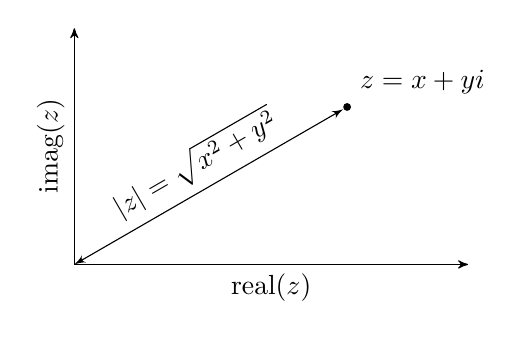
\begin{tikzpicture}
    \draw [-stealth'] (0, 0) -- ++(0:5) node [below,pos=0.5] {$\operatorname{real}(z)$};
    \draw [-stealth'] (0, 0) -- ++(90:3) node [above,pos=0.5,rotate=90] {$\operatorname{imag}(z)$};
    \node [point,label={above right:$z=x+yi$}] at (30:4) (1) {};
    \draw [latex'-latex'] (0, 0) -- node [above,rotate=30] {$|z|=\sqrt{x^2+y^2}$} (1);
\end{tikzpicture}
 
\end{document}